\section{Authentication}
\label{sec:authentication}

\subsection{Mechanism}
\status{IMPLEMENTED}

Stateless JWT authentication. Registration and login are handled by \pathref{backend/src/main/java/com/example/lms/controller/AuthController.java} and \pathref{backend/src/main/java/com/example/lms/service/AuthService.java}. Passwords are hashed with BCrypt; on success the backend issues a signed JWT (JJWT 0.12.6, secret \code{JWT_SECRET}, expiry \code{JWT_EXPIRATION=86400000} per \pathref{.env.example}). The frontend stores the token in \code{localStorage} (\pathref{frontend/src/context/AuthContext.jsx}) and attaches \code{Authorization: Bearer <token>} via an Axios interceptor (\pathref{frontend/src/api/client.js}).

\begin{figure}[H]
\centering
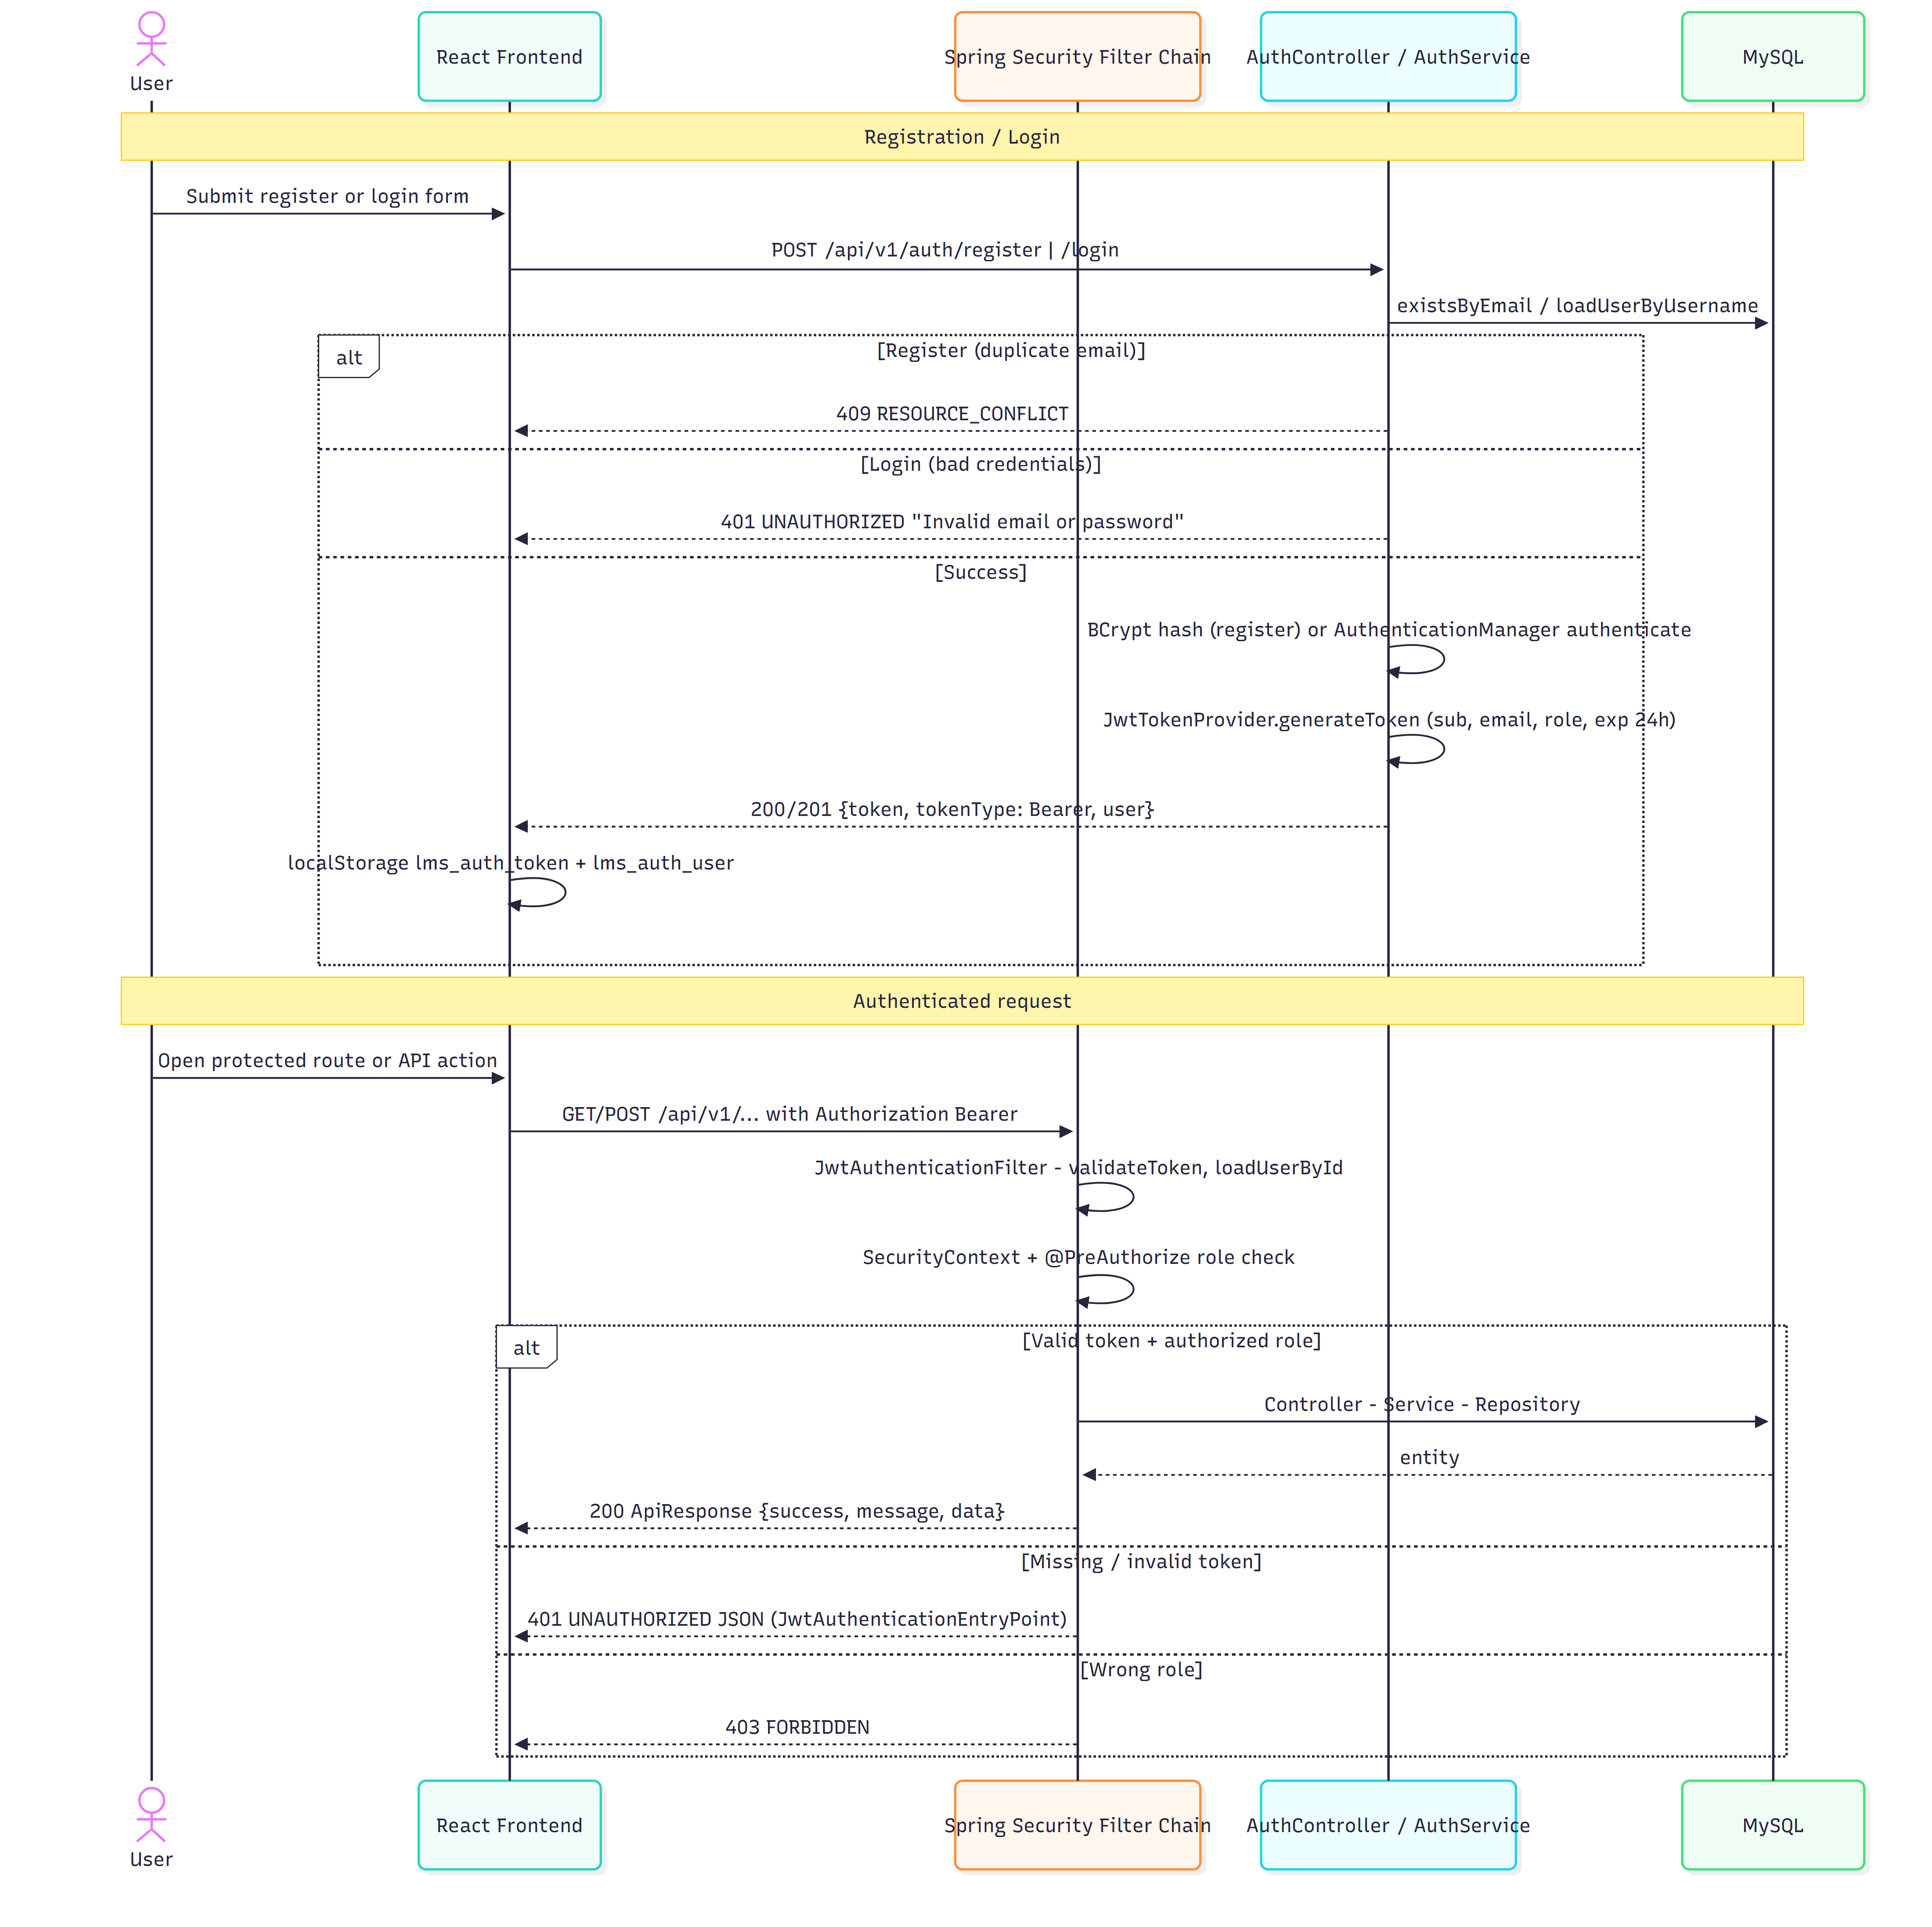
\includegraphics[width=0.95\textwidth]{diagrams/authentication-flow.png}
\caption{Authentication flow -- register, login, JWT issuance, per-request validation}
\label{fig:auth-flow-detail}
\end{figure}

\subsection{Validation chain}
\status{IMPLEMENTED}

Every request passes through the Spring Security filter chain (\pathref{backend/src/main/java/com/example/lms/config/SecurityConfig.java} plus \pathref{backend/src/main/java/com/example/lms/security/}): token signature and expiry are validated, the user principal is loaded, and method-level rules are applied. Invalid or expired tokens yield 401. There is no server-side session store and no token revocation list -- logout is client-side token removal plus a \code{POST /api/v1/auth/logout} acknowledgement.

\subsection{Limitations}
\status{IMPLEMENTED (gaps recorded)}

No password recovery, no email verification, no refresh-token rotation, and no lockout after repeated failures. Seed users created by \pathref{backend/src/main/java/com/example/lms/config/DataInitializer.java} use hardcoded passwords (finding S-02, Section~\ref{sec:security}).
